\documentclass{beamer}

% You can also use a 16:9 aspect ratio:
%\documentclass[aspectratio=169]{beamer}
\usetheme{TACC16}

% It's possible to move the footer to the right:
%\usetheme[rightfooter]{TACC16}

\begin{document}
\title[Lmod]{SC 22 Booth Talk: Lmod}
\author{Robert McLay} 
\date{Nov. 15, 2022}

% page 1
\frame{\titlepage} 

\section{Introduction}

% page 2
\begin{frame}{Introduction}
  \center{\includegraphics[width=.9\textwidth]{Lmod-4color@2x.png}}
  \begin{itemize}
    \item Features and History
    \item Advanced Topics
    \item Future work?
  \end{itemize}
\end{frame}

% page 3
\begin{frame}{Features}
  \begin{itemize}
    \item Current version is Lmod 8.7.14
    \item Reads for TCL and Lua modulefiles
    \item One name rule.
    \item Support Software Hierarchy (but not required!)
    \item Spider Cache: fast \texttt{\color{blue} \$ module avail}
    \item Properties (gpu, mic)
    \item family(``compiler'') family(``mpi'') support
    \item Optional Tracking: What modules are loaded?
    \item Many other features: ml, collections, hooks,
      extended default, nag ...
    \item Google analytics report about 2000 unique users around the
      world read docs every month.
  \end{itemize}
\end{frame}

% page 4
\begin{frame}{\texttt{Recent Feature of Lmod 8+}}
  \begin{itemize}
    \item The TCL interpreter is now (optionally) embedded with Lmod.
    \item \texttt{depends\_on()}
    \item New Function: \texttt{extensions("numpy/1.16.4 scipy/1.4")}
    \item Checking your module tree 8.4.3+
  \end{itemize}
\end{frame}

% page 5
\begin{frame}{\texttt{depends\_on()}}
  \begin{itemize}
    \item Modules X and Y depends on Module A
    \item ml purge; ml X; ml unload X;      $\Rightarrow$ unload A
    \item ml purge; ml X Y; ml unload X;    $\Rightarrow$ keep A
    \item ml purge; ml X Y; ml unload X Y ; $\Rightarrow$ unload A
    \item ml purge; ml A X Y; ml unload X Y ; $\Rightarrow$ keep A
  \end{itemize}
\end{frame}

% page 6
\begin{frame}{extensions() function}
  \begin{itemize}
    \item extensions(): Tells users that a module has extensions
    \item E.G: python has numpy and scipy
    \item \texttt{extensions("numpy/1.16.4, scipy/1.4")}
  \end{itemize}
\end{frame}

% page 7
\begin{frame}{extensions() function (II)}
  \begin{itemize}
    \item Users can use spider to find extensions.
    \item Users can use avail to list extensions base name
  \end{itemize}
\end{frame}

% page 8
\begin{frame}{Checking your module tree 8.4.3+}
  \begin{itemize}
    \item New command added: \texttt{\$LMOD\_DIR/check\_module\_tree\_syntax}
    \item Reports syntax errors across the entire \texttt{\$MODULEPATH}
    \item Report which modules have multiple marked defaults sets
    \item Precedent order: default symlink, .modulerc.lua, .modulerc, .version
    \item Does not check SYSTEM MODULERCFILE for defaults.
  \end{itemize}
\end{frame}

% page 9
\begin{frame}{Lmod 8.6+ Features}
  \begin{itemize}
    \item New Features now reported:
      https://lmod.readthedocs.io/en/latest/025\_new.html
    \item \texttt{module overview}
    \item \texttt{module -d avail}
    \item New config file: /etc/lmod/lmod\_config.lua
    \item LMOD\_QUARANTINE\_VARS
    \item updates to sh\_to\_modulefile
    \item source\_sh(): source a shell script inside a modulefile
  \end{itemize}
\end{frame}

% page 10
\begin{frame}[fragile]
  \frametitle{module overview}
    {\tiny
\begin{semiverbatim}
% module overview
------------------ /opt/apps/modulefiles/Core -----------------
StdEnv    (1)   hashrf    (2)   papi        (2)   xalt     (1)
ddt       (1)   intel     (2)   singularity (2)
git       (1)   noweb     (1)   valgrind    (1)

--------------- /opt/apps/lmod/lmod/modulefiles/Core ----------
lmod (1)   settarg (1)    
\end{semiverbatim}
    }
\end{frame}

% page 11
\begin{frame}{\$LMOD\_QUARANTINE\_VARS}
  \begin{itemize}
    \item A module at TACC turn-off  \$LMOD\_PAGER
    \item This \!\@\#\%\& module made me mad.
    \item Tmod has a new feature kinda like this.
    \item \$LMOD\_QUARANTINE\_VARS was invented.
  \end{itemize}
\end{frame}

% page 12
\begin{frame}{\$LMOD\_QUARANTINE\_VARS (II)}
  \begin{itemize}
    \item export LMOD\_QUARANTINE\_VARS=LMOD\_PAGER:LMOD\_REDIRECT
    \item This means that a module can't change those variables.
    \item This only works with regular env. vars.
    \item You can't quarantine PATH like variables.
    \item A user sets this variable in their $\sim$/.bashrc or similar
      file.
    \item This obviously won't work for modules loaded during the
      processing of /etc/profile.d/*.sh files
    \item Use https://github.com/TACC/ShellStartupDebug support users.
  \end{itemize}
\end{frame}

% page 13
\begin{frame}[fragile]
  \frametitle{/etc/lmod/lmod\_config.lua configuration file}
  \begin{itemize}
    \item This file is evaluated during Lmod startup. 
    \item This location is the default during configuration.
    \item A site can change this location at configuration.
  \end{itemize}
    {\small
\begin{semiverbatim}
-- Example /etc/lmod/lmod\_config.lua
require("strict")
local cosmic = require("Cosmic"):singleton()

cosmic:assign("LMOD\_SITE\_NAME", "XYZZY")
local function foo()
  ...
end
sandbox\_registration \{ foo = foo \}
\end{semiverbatim}
}
\end{frame}

% page 14
\begin{frame}{Sourcing shell scripts inside a modulefile w/ source\_sh()}
  \begin{itemize}
    \item This was first implemented in Tmod 4.7
    \item Xavier told me that he did this during Covid Lockdown in France.
    \item Lmod 8.6 re-implements this feature in a similar way.
    \item It knows about env. vars and shell functions and aliases.
  \end{itemize}
\end{frame}

% page 15
\begin{frame}{source\_sh() Implementation}
  \begin{itemize}
    \item It captures the env. vars/functions/alias before and after
      the running the shell script.
    \item It computes the difference and saves it into the ModuleTable
      in env.
    \item It can be safely unloaded, shown.
    \item script path and arguments must not change between load and unload.
    \item \texttt{module refresh} works
    \item Obvious points:
      \begin{itemize}
        \item It is better to use sh\_to\_modulefile and convert once.
        \item But sh\_to\_modulefile is not dynamic (e.g. \$HOME)
        \item Can't have run the script in the user environment before
          loading the script.
      \end{itemize}
  \end{itemize}
\end{frame}

% page 16
\begin{frame}[fragile]
  \frametitle{ml --mt}
    {\tiny
\begin{semiverbatim}
\_ModuleTable\_ = \{
  MTversion = 3,
  mT = \{
    wrapperSh = \{
      fn = "/home/user/w/lmod/rt/sh_to_modulefile/mf/wrapperSh/1.0.lua",
      fullName = "wrapperSh/1.0",
      loadOrder = 1,
      mcmdT = {
        ["/home/user/w/lmod/rt/sh_to_modulefile/second.sh arg1"] = \{
          "setenv(\\"SECOND\\",\\"FOO_BAR\\")",
        \},
        ["/home/user/w/lmod/rt/sh_to_modulefile/tstScript.sh"] = \{
          "setenv(\\"MY_NAME\",\\"tstScript.sh\\")",
          "prepend_path(\\"PATH\\",\\"/home/user/w/lmod/rt/sh_to_modulefile/bin\\")",
          "set_alias(\\"fooAlias\\",\\"foobin -q -l\\")"
          , [[set_shell_function("banner"," \\
    local str=\\"$1\\";\\
    local RED='\\27[1;31m';\\
    local NONE='\\27[0m';\\
    echo \\"${RED}${str}${NONE}\\"\\
")]], 
        \},
      \},
    \},
  \},
}
\end{semiverbatim}
    }
\end{frame}

% page 17
\begin{frame}{Lmod Monthly Zoom Mtg}
  \begin{itemize}
    \item Previous Topics
      \begin{enumerate}
        \item Lmod Hooks Discussion
        \item Debugging Modulefiles
        \item Lmod 8.6 new features
        \item Settarg and integrating Lmod with build system
        \item How Module collections works 
        \item How to get current module info into hooks
        \item How Lmod testing works
      \end{enumerate}
    \item Future Topics: 
      \begin{enumerate}
        \item How TCL modules are interpreted
      \end{enumerate}
    \item Zoom Mtg Usually 1st Tuesday at 15:30 UTC (9:30 US Central)
    \item See Mailing list or https://github.com/TACC/Lmod/wiki for
      details
    \item Next Meeting Dec. 6th at 15:30 UTC (9:30 US Central)
  \end{itemize}
\end{frame}

% page 18
\begin{frame}[fragile]
    \frametitle{Lmod Doc usage by City}
    \center{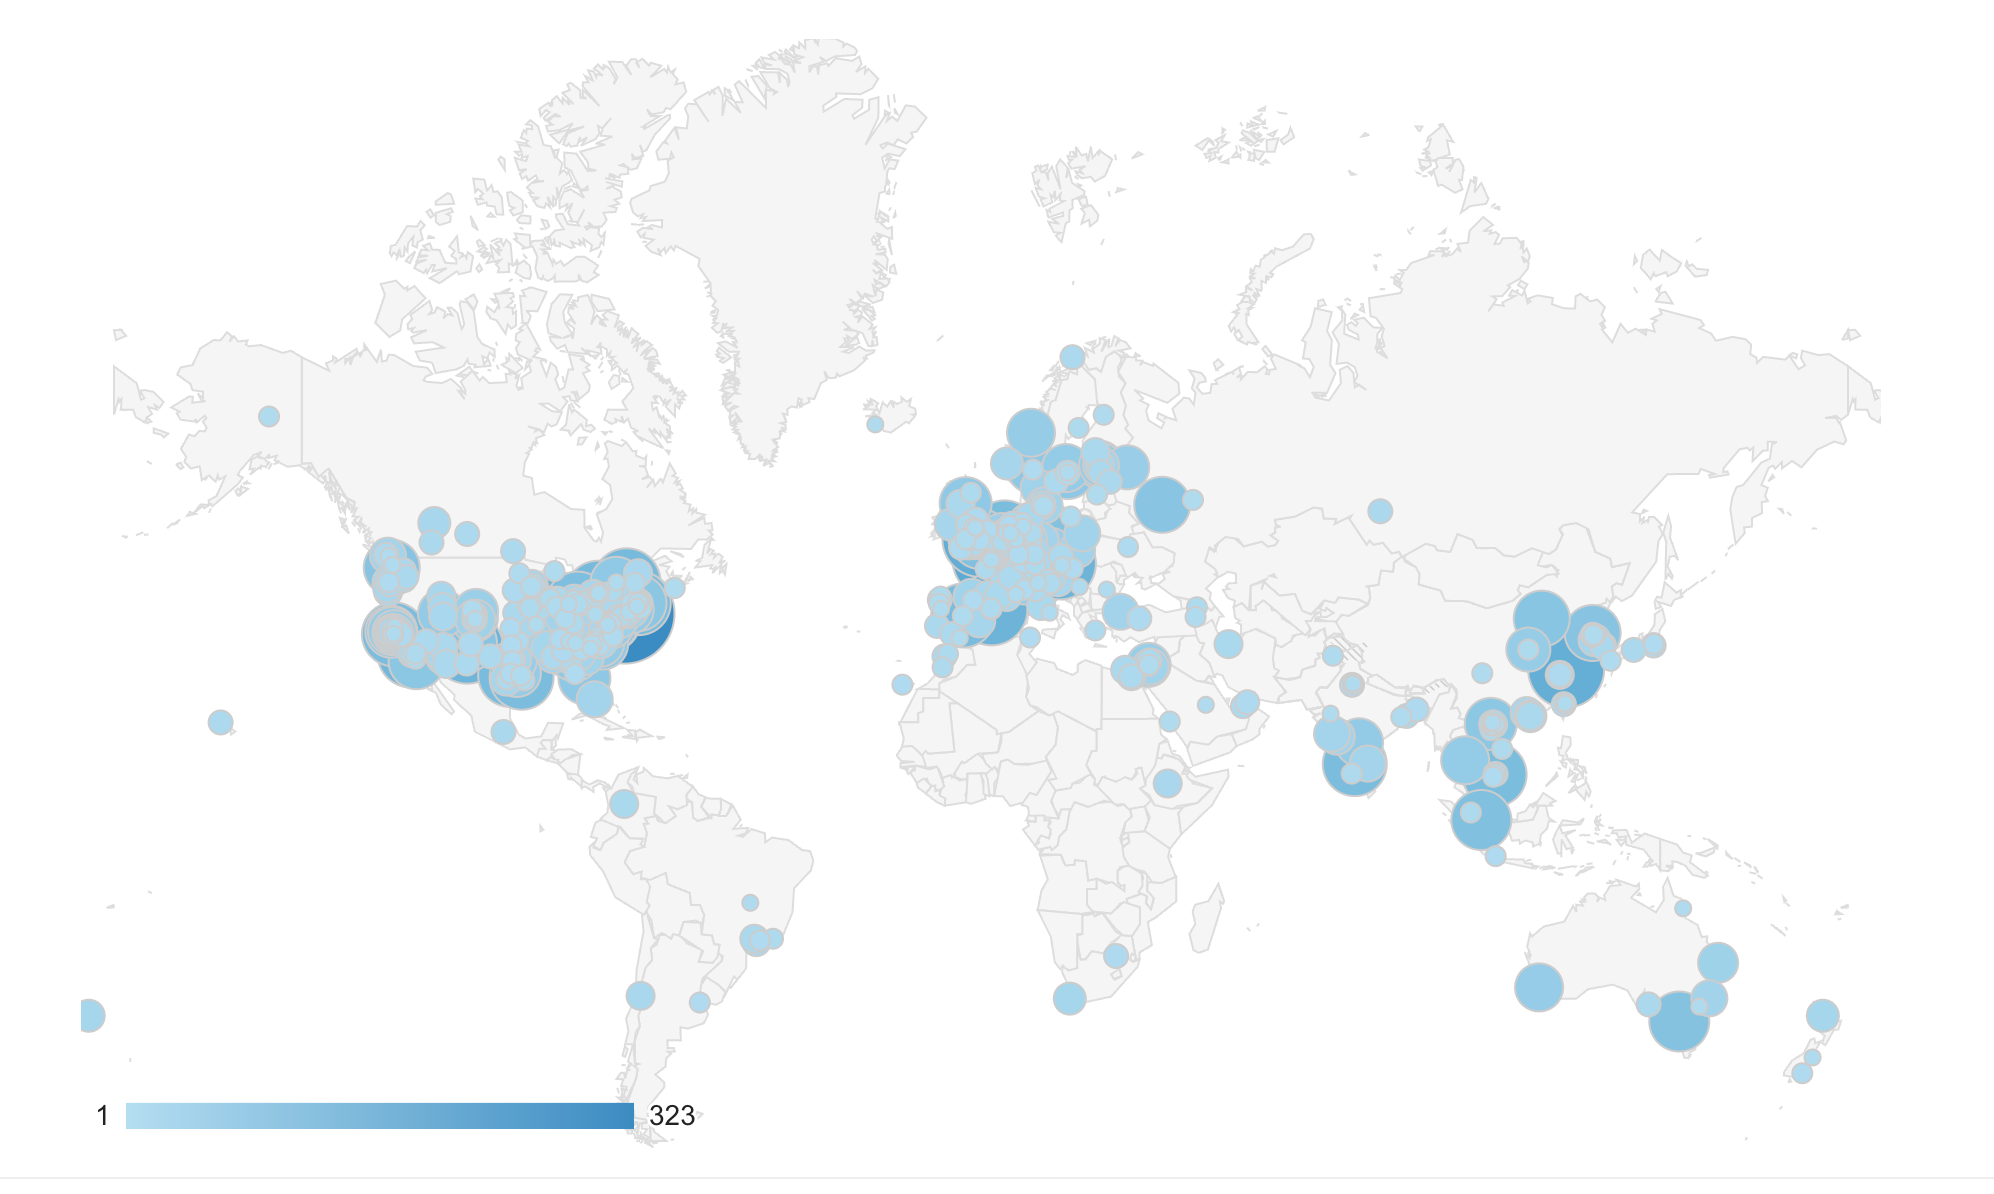
\includegraphics[width=.9\textwidth]{Lmod_doc_usage_by_city}}
\end{frame}

% page 19
\begin{frame}[fragile]
    \frametitle{Lmod Doc usage by Country}
    \center{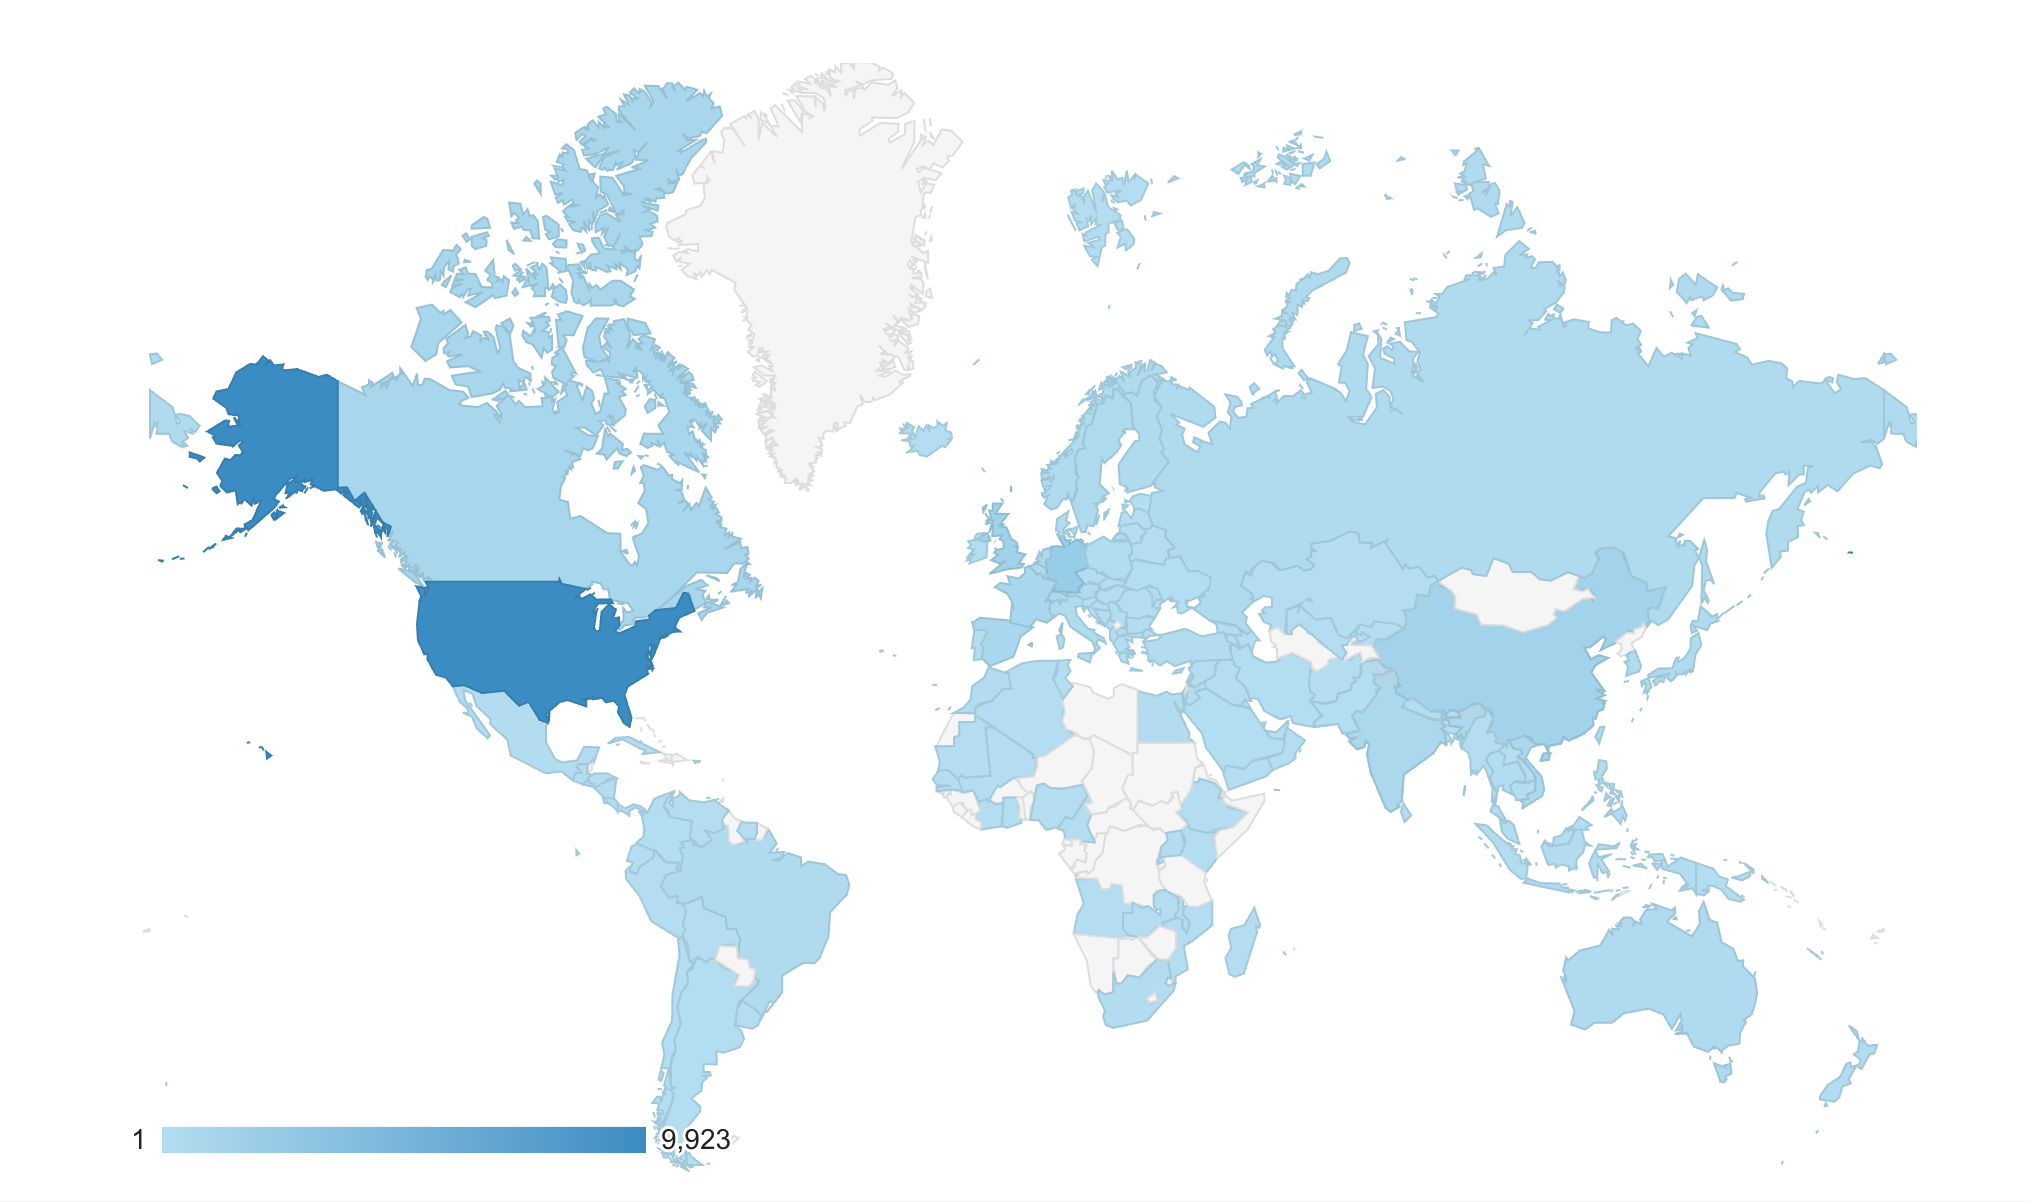
\includegraphics[width=.9\textwidth]{Lmod_doc_usage_by_country}}
\end{frame}

% page 20
\begin{frame}{Future Work}
  \begin{itemize}
    \item Lmod can optionally track usage.
    \item Future: Make it easier to not remember loads after 1 year.
    \item A monthly discussion group? (YES!!)
    \item Remember text of modules to unload.
  \end{itemize}
\end{frame}

% page 21
\begin{frame}{Conclusions: Lmod 8+}
  \center{\includegraphics[width=.9\textwidth]{Lmod-4color@2x.png}}
  \begin{itemize}
    \item Latest version: https://github.com:TACC/lmod.git
    \item Stable version: http://lmod.sf.net
    \item Documentation:  http://lmod.readthedocs.org
    \item Talks:          https://github.com/xalt/xalt/tree/main/my\_docs/22
  \end{itemize}
\end{frame}

\end{document}
